
\section{Introduzione}
\nsub{Obiettivi}
\small{Che caratteristiche vorremmo da un polimero coniugato {\bf donatore} che sia utilizzabile in una cella solare?
\begin{itemize}
 \item Energia del HOMO adatta all'uso con un materiale accettore;
 \item intenso assorbimento luminoso su tutto lo spettro solare;
 \item coniugazione che permette alta mobilità di lacune intracatena; 
 \item cristallinità per mobilità di lacune intercatena (che permette celle più spesse) ed aggiunge nuove bande di assorbimento;
 \item decadimento lento degli eccitoni e assenza di ricombinazione di cariche;
  \item morfologia \emph{bulk heterojunction};
\item solubilità e processabilità per formare film;
 \item stabilità chimica e morfologica;
 \item economicità.
\end{itemize}}

\end{frame}
%%%%%%%%%%%%%%%%%%%%%%%%%%%%%%%%%%%%%%%%%%%%%%%%%%%%%%%%%%%%%%%%%%%%%%%%%%%%%%%%%%%%%%%%%%%%%%%%%%%%%%%%%%%%%%%%%%%%%%%%%%%%%%
\nsub{Livelli energetici} %fv-eccit

\begin{columns}
\column{0.6\linewidth}
Vorremmo:
\begin{itemize}
  \item $E_g$ piccolo per assorbire una maggiore porzione dello spettro solare: $2eV => 30\%$ dello spettro;% \cite{fv-eccit}
  \item $E_d \geq 0.3eV$ \emph{driving force} per spezzare l'eccitone;
  \item $V_{built-in}$ grande, corrisponde al massimo $V_{open-circuit}$;
\end{itemize}
quindi è necessario un compromesso:\\ si ritiene 1.4eV essere il \emph{band gap} ottimale.%\cite{conj-sint}
\column{0.3\linewidth} \begin{figure}{\centering{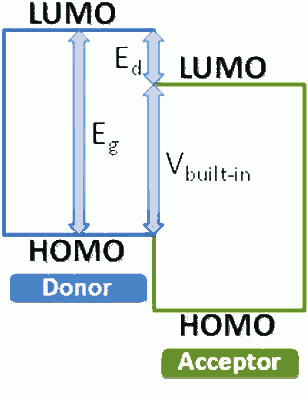
\includegraphics[width=1\textwidth]{img/lvl_energ.png}}}\end{figure}
\end{columns}
\end{frame}

\subsubsection{Band Gap}\begin{frame}\frametitle{Livelli energetici}\framesubtitle{Band Gap}

Per avere un basso $E_g$ ossia il \emph{band gap}:
\begin{itemize}
    \item minore aromaticità dei monomeri dunque maggiore peso della forma chinonica e maggiore coniugazione;
  \end{itemize} \begin{columns}
\column{0.7\linewidth}  \begin{itemize}\item planarità ad es. meno repulsione catene laterali o usando monomeri policiclici;
    \item il \emph{band gap} non decresce allungando oltre una ventina di monomeri coniugati;
    \item sostituenti elettron-donatori alzano HOMO, elettron-attrattori abbassano LUMO.
 \end{itemize}
\column{0.4\linewidth}\vspace{-20pt}\begin{figure}{\centering{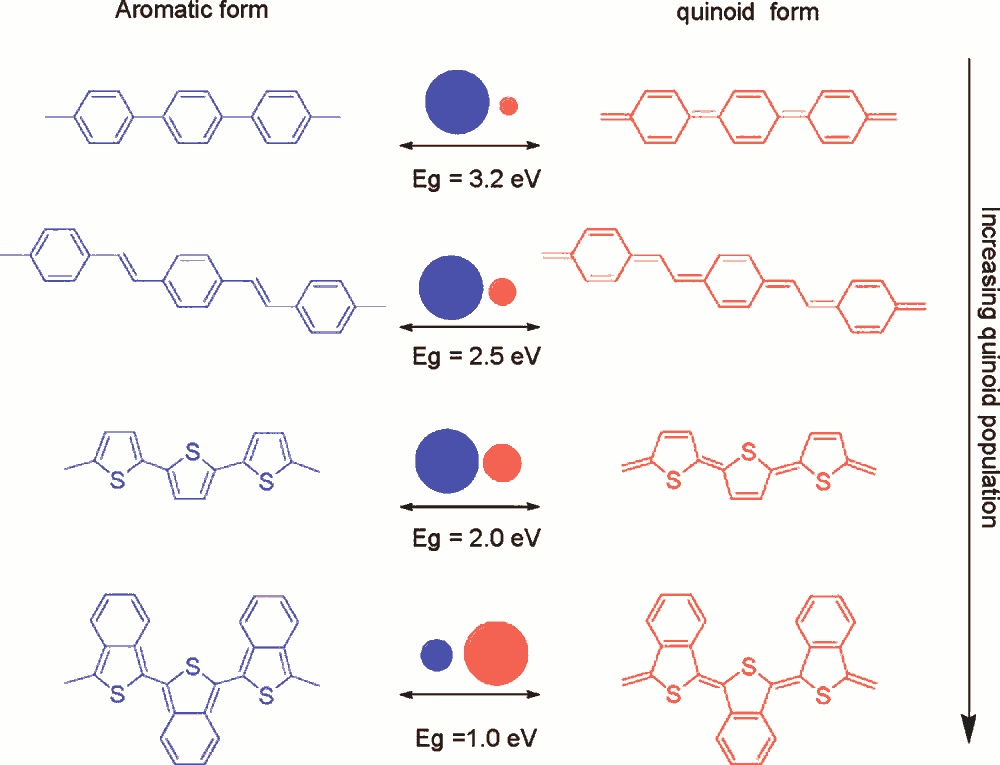
\includegraphics[width=1\textwidth]{img/chinoni.png}}}\end{figure}

\end{columns}\vspace{-10pt}\begin{figure}{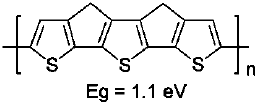
\includegraphics[width=0.25\textwidth]{img/tiofeniplanari.png}\hspace{20pt}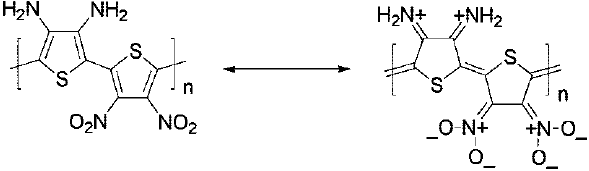
\includegraphics[width=0.5\textwidth]{img/dimero.png}}\end{figure}\end{frame}
%%%%%%%%%%%%%%%%%%%%%%%%%%%%%%%%%%%%%%%%%%%%%%%%%%%%%%%%%%%%%%%%%%%%%%%%%%%%%%%%%%%%%%%%%%%%%%%%%%%%%%%%%%%%%%%%%%%%%%%%%%%%%%
\nsub{Solubilità}
Per ottenere solubilità e quindi processabilità si può manipolare:
\begin{itemize}
    \item lunghezza delle catene laterali alifatiche meglio se ramificate (diminuiscono il $\pi-\pi$ \emph{stacking}) però diminuiscono la conducibilità intercatena;
        \item interazioni intermolecolari ($\pi-\pi$ \emph{stacking});
\item polarità delle catene laterali;
\item grado di polimerizzazione;
    \item rigidità e regioregolarità della catena principale.
  \end{itemize}

\end{frame}
%%%%%%%%%%%%%%%%%%%%%%%%%%%%%%%%%%%%%%%%%%%%%%%%%%%%%%%%%%%%%%%%%%%%%%%%%%%%%%%%%%%%%%%%%%%%%%%%%%%%%%%%%%%%%%%%%%%%%%%%%%%%%%
\nsub{Sintesi in generale}
\begin{columns}\column{0.5\linewidth} 

Le reazioni di \emph{coupling} mediate da metalli di transizione permettono di creare nuovi legami Csp$^2$-Csp$^2$ e Csp$^2$-Csp.

Molte di queste reazioni possono essere utilizzate per ottenere polimeri coniugati.
\column{0.5\linewidth} 
\begin{figure}{\centering{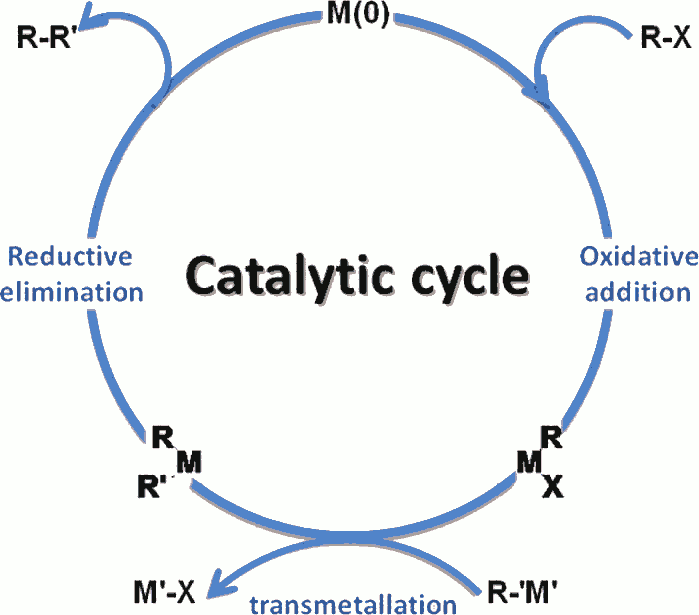
\includegraphics[width=0.7\textwidth]{img/cross-coupling.png}}}\end{figure}
\end{columns}
\vspace{15pt}
Per alcuni polimeri coniugati sono state sviluppate polimerizzazioni viventi per avere bassa polidispersità.
\end{frame}
%%%%%%%%%%%%%%%%%%%%%%%%%%%%%%%%%%%%%%%%%%%%%%%%%%%%%%%%%%%%%%%%%%%%%%%%%%%%%%%%%%%%%%%%%%%%%%%%%%%%%%%%%%%%%%%%%%%%%%%%%%%%%%
\nsub{Reazioni di polimerizzazione}\footnotetext{\tiny{\cite{conj-sint}DOI: 10.1021/cr900182s}}
Esempi di reazioni da monomeri a polimeri coniugati (ed esempi):
\small{
\begin{itemize}
 \item Suzuki (\ce{(R'O)2B-R-B(OR')2}, dibromuro, \ce{Pd(PPh3)4});
 \item Yamamoto (dibromuro, \ce{Ni(COD)2}, bpy);
 \item Stille (dibromuro, \ce{Me3Sn-R-SnMe3}, \ce{Pd(PPh3)4});
 \item Sonogashira (dibromuro, dialchino, \ce{Pd(PPh3)4}, \ce{CuI}, \ce{R2NH});
 \item Heck (\ce{H2C=CH-R-Br}, \ce{Pd(OAc)2}, \ce{PR3});
 \item GRIM e Kumada-Corriu (dibromuro, \ce{RMgX}, \ce{Ni(dppp)Cl2});
 \item Knoevenagel (dialdeide, dinitrile, \ce{t-BuOK});
 \item Wittig-Horner (dialdeide, \ce{(EtO)2OP-R-PO(OEt)2}, \ce{t-BuOK});
 \item polimerizzazione elettrochimica;
 \item polimerizzazione termica;
 \item polimerizzazione ossidativa con \ce{FeCl3}.
\end{itemize}
}
\end{frame}

%%%%%%%%%%%%%%%%%%%%%%%%%%%%%%%%%%%%%%%%%%%%%%%%%%%%%%%%%%%%%%%%%%%%%%%%%%%%%%%%%%%%%%%%%%%%%%%%%%%%%%%%%%%%%%%%%%%%%%%%%%%%%%
%%%%%%%%%%%%%%%%%%%%%%%%%%%%%%%%%%%%%%%%%%%%%%%%%%%%%%%%%%%%%%%%%%%%%%%%%%%%%%%%%%%%%%%%%%%%%%%%%%%%%%%%%%%%%%%%%%%%%%%%%%%%%%
%%%%%%%%%%%%%%%%%%%%%%%%%%%%%%%%%%%%%%%%%%%%%%%%%%%%%%%%%%%%%%%%%%%%%%%%%%%%%%%%%%%%%%%%%%%%%%%%%%%%%%%%%%%%%%%%%%%%%%%%%%%%%%
